\chapter{Electric Vehicles}
\label{ch:elvehicles}
% ##################################################################################################################

\hfill \textbf{Author:} Rashid A. Waraich, Joschka Bischoff

\begin{center} 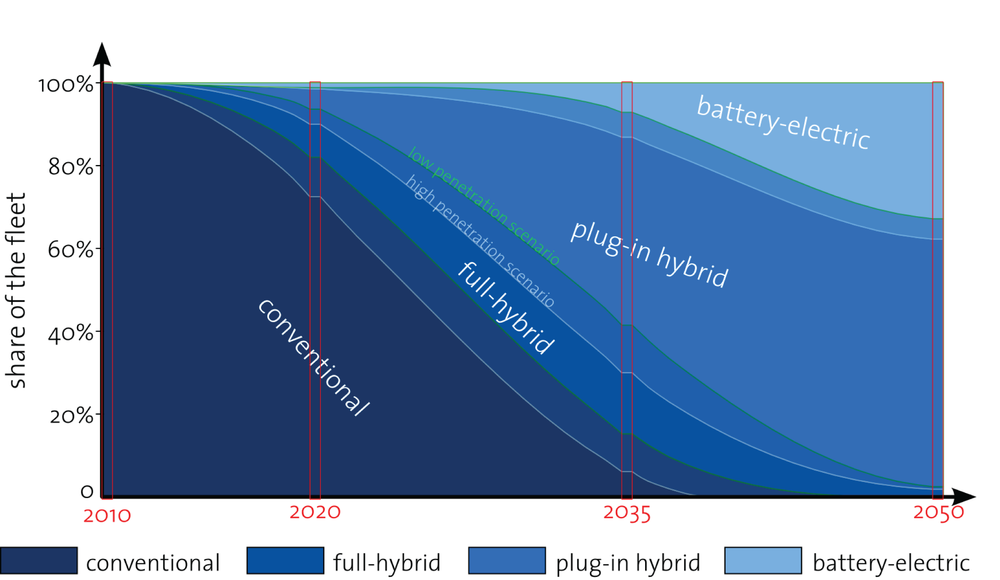
\includegraphics[width=0.65\textwidth, angle=0]{extending/figures/Elvehicles/main.png} \end{center}

\editdone{This text has undergone the professional edit. Please no grammatical changes anymore! They are most-probably wrong.}

\createStandardInformationBasic{transEnergySim}{No predefined invocation. A starting point is \lstinline|RunTransEnerySimExample| class}{No typical \gls{matsim} config}{\citet[][]{WaraichEtAl_TRR_2013, GalusEtAl_STRC_2009, WaraichEtAl_IATBR_2009, GalusEtAl_ITSG_2012, Waraich_PhDThesis_2014, AbedinWaraich_TechRep_IVT_2013, WaraichEtAl_TechRep_IVT_2013, GalusEtAl_ResRep_EWZ_2012, Waraich_unpub_EURO_2012, Waraich_unpub_MATSimUserMeeting_2012, WaraichEtAl_JanssensEtAl_2014, WaraichAxhausen_SDEWES_2013}}
\joschka{Verwende basic, da es kein config-basiertes Modul ist.}

% ##################################################################################################################
\section{Introduction}
Research related to \gls{ev} modeling in \gls{matsim} started in 2008/2009, with an electricity grids project \citep[][]{WaraichEtAl_IATBR_2009, WaraichEtAl_TRR_2013}; it's goal was to uncover potential bottlenecks and/or constraint violations in Zurich city's lower voltage grid due to future \gls{ev} charging. A framework emerged from the research for \gls{ev} modeling, called \gls{tesf} \citep[][]{WaraichEtAl_JanssensEtAl_2014}. This resulted in various framework extensions and enabled simulation of various scenarios \citep[][]{WaraichEtAl_JanssensEtAl_2014, Waraich_PhDThesis_2014, AbedinWaraich_JSDEWES_2014, Schieffer_MastersThesis_2011, GalusAndersson_CIGRE_2011, GalusEtAl_ResRep_EWZ_2012, Bischoff2013MaTaxis and BischoffMaciejewskiEcabMielecMobilTUM}. This chapter provides advice on these research directions and serves as a starting point for modeling \glspl{ev} in \gls{matsim}.

% ##################################################################################################################
\section{Models}
The main reason for modeling \glspl{ev} in \gls{tesf} was simple: it was essential to keep track of the battery charging state in the \glspl{ev}. This meant that, as the \gls{ev} was driving, depletion of the batteries was simulated. It was also important to consider the charging process of \glspl{ev} at charging infrastructures.

While the basic \gls{ev} modeling mechanisms were simple, there were many details to ponder when modeling scenarios. 
The \gls{tesf} framework provided both interfaces and implementations to cope with more complex cases, \eg defining a vehicle that can charge without contact while driving,
\karen{Is this last phrase correctly changed? The wording was confusing for me... Thanks!} \ah{I would say: yes}
for example, by using dynamic inductive charging. Furthermore, charging mechanisms themselves could also be quite complex. The following sections provided some details on this, as well as different models involved.

% ==============================================================================================
\subsection{Energy Consumption Model}
When a vehicle was defined in \gls{tesf}, it could be assigned an energy consumption model, defining how much energy the vehicle used while driving. For conventional vehicles, just energy consumption could be logged using such a model; however, for electric vehicles, the energy consumption model was used to update the on-board battery system state of charge. \glspl{phev} can use both electricity and gasoline for driving and therefore had two different energy consumption models assigned to them for modeling these two modes. When this was written, a series hybrid model were implemented in \gls{tesf} \citep[][]{Chan_PIEEE_2007}, which used electricity as long as the battery charge state was above a certain threshold value, then switched to gasoline. This type of vehicle could also be charged using a plug, like a battery electric vehicle. For \glspl{phev}, car manufacturers often defined rules governing when a vehicle should switch between battery and gasoline use. The \gls{tesf} framework provided interfaces and examples of how more advanced control strategies for \glspl{phev} could be implemented.

% ==============================================================================================
\subsection{Charging Infrastructure}
In addition to plug-based charging, inductive charging infrastructure was also modeled in \gls{tesf}, with two types: dynamic and stationary. The dynamic inductive charging infrastructure was often embedded in roads; vehicles able to use such infrastructure could charge while they drove. Stationary inductive charging was, more or less, modeled like plug charging; however, charging interfaces between vehicle and the charging infrastructure had to match for the charging process to function.

Another fast route to a full battery was to replace/swap the used battery for a new one at a specialized infrastructure, sometimes referred to as a swapping station \citep[][]{LiEtAl_ACC_2011}. A basic modeling of this approach was provided in \gls{tesf}, which could be extended and detailed further according to specific scenario needs.

% ==============================================================================================
\subsection{Charging Schemes}
When an \gls{ev} connected to any infrastructure for charging, a scheme was needed to define how the vehicle charging would operate; should the vehicle start charging immediately, or would charging depend on an agent's pricing preferences, which could vary with time and location? Negotiations between the vehicle computer and grid operator were also possible, which perhaps allowed for some electricity grid temporal flexibility, while fully charging a vehicle's battery before departure (sometimes referred to as ``smart charging''). Various charging schemes were part of the \gls{tesf} and were be used to model other more complex charging schemes; \gls{tesf}-simulated examples of various charging schemes can be found in \citet[][]{WaraichEtAl_TRR_2013}.

% ==============================================================================================
\subsection{\protect\gls{v2g}}
When studying electric vehicles, charging is not the only topic of interest; \gls{v2g} applications where electric vehicle batteries supply power and energy back to the grid \citep[][]{KemptonTomic_JPS_2005} were analyzed. While the integration of \gls{v2g} models for \gls{matsim} was limited at any given time, an application related to \gls{v2g} and intermittent energy generation at wind parks using \gls{matsim} can be found in \citet[][]{GalusAndersson_CIGRE_2011} and a preliminary attempt to integrate \gls{v2g} in \gls{tesf} was described in \citet[][]{WaraichEtAl_JanssensEtAl_2014, Schieffer_MastersThesis_2011}.

% ==============================================================================================
\subsection{Vehicle Choice}
When conducting electric vehicle studies, each vehicle owner usually has to be assigned a specific type: \eg electric vehicle, conventional vehicle, plug-in hybrid, etc. Sometimes, these assignments were random, while ensuring vehicle type share constraints for the scenario \citep[e.g.,][]{WaraichEtAl_JanssensEtAl_2014}. Often, however, possible financial or infrastructural incentive implications, \eg different toll prices, parking fees or fuel prices for different vehicle types, had to be evaluated. A replanning module for vehicle choice, also covering \glspl{ev}, was recently implemented; first results should published soon and can also be integrated in \gls{tesf}.

This section provided an overview of the various \gls{tesf} framework parts and the following section an application of a \gls{tesf} extension, that modeled electric taxis.

% ##################################################################################################################
\section{Application: Electric Taxis} % Author: Joschka Bischoff
Combination and extension of both the \gls{tesf} and \gls{vrp} contribution (see Chapter~\ref{ch:dts}) allows simulation of \glspl{bev} taxi fleets.
For electric vehicles, vehicle charging process was adapted; for taxis, the concept of taxi ranks and a modified optimizer sending idling taxis to the rank and only dispatching vehicles with sufficient battery charge were introduced. 

% ==============================================================================================
\subsection{Taxi Ranks}
After dropping off passengers, taxis proceeded to the nearest rank location, unless there was an immediate follow-up request. 
Queuing took place at the rank location; the taxi that arrived first would leave the rank first. 
Other types of queuing were also tested, \eg a dispatch by battery \gls{soc}.
Ranks were not mandatory; however, driving there between trips would be typical German taxi driver behavior.

% ==============================================================================================
\subsection{Charging Process}
Chargers could be located at taxi ranks or any other link. 
Following any given \gls{bev} \lstinline$AgentArrivalEvent$ at a charger location link, charging would begin if
%
\begin{compactitem}
	\item there was a free charging spot,
	\item the vehicle's \gls{soc} was under a certain threshold,
	\item at least two minutes of time passed required for parking the car and plugging it in.
\end{compactitem}

Electric taxi simulation has been used in Mielec, Poland \citep[][]{Bischoff2013MaTaxis, BischoffMaciejewskiEcabMielecMobilTUM}. When this was written, an application for Berlin was in progress.

% ##################################################################################################################
\section{Usage}
The \gls{tesf} \gls{contribution} contained many features described above and interfaces were provided for framework extension. 
Examples were also given for the setup of different scenarios: \eg energy consumption model, vehicle types, charging schemes, etc.

% ##################################################################################################################

